%%Copyright 2021. Any replication of this document is permissible. The primary package of this document is from cjquines%%

%%PRIMARY PREAMBLE%%
\documentclass[11pt,paper=letter]{scrartcl}
\usepackage[boxthm, wide]{cjquines}
\usepackage{CJKutf8}
\usepackage{jrobaob}
\usepackage{soul}
\usepackage{color}
\usepackage[usenames,dvipsnames]{xcolor}

\newcommand{\hlc}[2][yellow]{ {\sethlcolor{#1} \hl{#2}} }


\begin{document}


\title{Integration: The Tic Tac Toe Method}
\subtitle{\joshbluebf{Ateneo De Davao University Senior High School}}
\author{Josh Robert D. Obaob}
\date{March 15, 2022}

\maketitle




\begin{abstract}
Most of the time, when we integrate an expression, we often use the \joshbf{u-substitution}. However, there are some instances that such method is useless to be applied on \textit{special} cases, say, "integrate $\int \left(x^4 \cos{x}\right) dx$." If you think about it, it is nearly impossible to integrate using the $u$-substitution since the situation is odd. Luckily, we have a remedy for and that is the \joshbluebf{Tic Tac Toe Method}. (\textbf{Disclaimer:} If you are not studying the u-substitution, then this module is \textbf{NOT} for you.)
\end{abstract}

\section{Definition}

The \joshbf{Tic-Tac-Toe Method} or the {tabular integration by parts method}. Such method is very powerful to use and it can almost integrate every expression you may faced! Using the method requires basic knowledge on higher-ordered derivatives because it is crucial to the efficiency of such method, otherwise, the method would not be working for you.

\begin{center}
    


\tikzset{every picture/.style={line width=0.75pt}} %set default line width to 0.75pt        

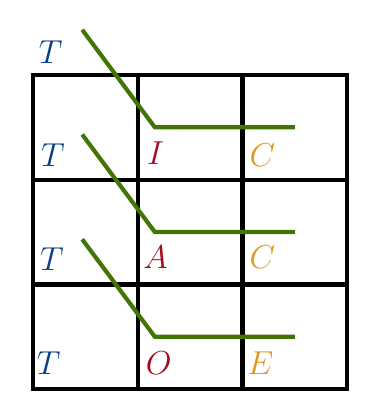
\begin{tikzpicture}[x=0.75pt,y=0.75pt,yscale=-1,xscale=1]
%uncomment if require: \path (0,300); %set diagram left start at 0, and has height of 300

%Shape: Rectangle [id:dp2754337250250303] 
\draw  [line width=1.5]  (239.17,171.33) -- (289.63,171.33) -- (289.63,221.8) -- (239.17,221.8) -- cycle ;
%Shape: Square [id:dp9079966809140174] 
\draw  [line width=1.5]  (289.63,171.33) -- (340.1,171.33) -- (340.1,221.8) -- (289.63,221.8) -- cycle ;
%Shape: Square [id:dp5777370022086523] 
\draw  [line width=1.5]  (239.17,120.87) -- (289.63,120.87) -- (289.63,171.33) -- (239.17,171.33) -- cycle ;
%Shape: Rectangle [id:dp7353124356190535] 
\draw  [line width=1.5]  (289.63,120.87) -- (340.1,120.87) -- (340.1,171.33) -- (289.63,171.33) -- cycle ;
%Shape: Rectangle [id:dp12928939553050722] 
\draw  [line width=1.5]  (188.7,171.33) -- (239.17,171.33) -- (239.17,221.8) -- (188.7,221.8) -- cycle ;
%Shape: Square [id:dp9109660927518908] 
\draw  [line width=1.5]  (188.7,120.87) -- (239.17,120.87) -- (239.17,171.33) -- (188.7,171.33) -- cycle ;
%Shape: Square [id:dp3316177859825151] 
\draw  [line width=1.5]  (239.17,70.4) -- (289.63,70.4) -- (289.63,120.87) -- (239.17,120.87) -- cycle ;
%Shape: Rectangle [id:dp8278102195962869] 
\draw  [line width=1.5]  (289.63,70.4) -- (340.1,70.4) -- (340.1,120.87) -- (289.63,120.87) -- cycle ;
%Shape: Square [id:dp5856168358096059] 
\draw  [line width=1.5]  (188.7,70.4) -- (239.17,70.4) -- (239.17,120.87) -- (188.7,120.87) -- cycle ;

%Straight Lines [id:da3045165412456208] 
\draw [color={rgb, 255:red, 65; green, 117; blue, 5 }  ,draw opacity=1 ][line width=1.5]    (212.37,48.63) -- (247.37,95.63) -- (314.87,95.63) ;
%Straight Lines [id:da030191021676013508] 
\draw [color={rgb, 255:red, 65; green, 117; blue, 5 }  ,draw opacity=1 ][line width=1.5]    (212.37,99.1) -- (247.37,146.1) -- (314.87,146.1) ;
%Straight Lines [id:da8286373782428256] 
\draw [color={rgb, 255:red, 65; green, 117; blue, 5 }  ,draw opacity=1 ][line width=1.5]    (212.37,149.57) -- (247.37,196.57) -- (314.87,196.57) ;

% Text Node
\draw (197.23,59.24) node  [font=\large,color={rgb, 255:red, 8; green, 64; blue, 131 }  ,opacity=1 ]  {$T$};
% Text Node
\draw (198.23,109.24) node  [font=\large,color={rgb, 255:red, 8; green, 64; blue, 131 }  ,opacity=1 ]  {$T$};
% Text Node
\draw (197.73,159.24) node  [font=\large,color={rgb, 255:red, 8; green, 64; blue, 131 }  ,opacity=1 ]  {$T$};
% Text Node
\draw (196.23,209.24) node  [font=\large,color={rgb, 255:red, 8; green, 64; blue, 131 }  ,opacity=1 ]  {$T$};
% Text Node
\draw (247.73,108.24) node  [font=\large,color={rgb, 255:red, 163; green, 11; blue, 30 }  ,opacity=1 ]  {$I$};
% Text Node
\draw (247.73,158.24) node  [font=\large,color={rgb, 255:red, 163; green, 11; blue, 30 }  ,opacity=1 ]  {$A$};
% Text Node
\draw (249.23,209.24) node  [font=\large,color={rgb, 255:red, 163; green, 11; blue, 30 }  ,opacity=1 ]  {$O$};
% Text Node
\draw (299.23,109.24) node  [font=\large,color={rgb, 255:red, 226; green, 152; blue, 30 }  ,opacity=1 ]  {$C$};
% Text Node
\draw (299.23,158.24) node  [font=\large,color={rgb, 255:red, 226; green, 152; blue, 30 }  ,opacity=1 ]  {$C$};
% Text Node
\draw (298.23,209.24) node  [font=\large,color={rgb, 255:red, 226; green, 152; blue, 30 }  ,opacity=1 ]  {$E$};


\end{tikzpicture}
\end{center}

Let us have some examples.



\section{Some Examples}

\subsection*{Example 1}

As I mentioned in my introduction, let us try to integrate or find the anti-derivative of $x^4 \cos x$ using the method.

\newpage

\begin{mdframed}[style=jradduemmdbox, frametitle=Example 1.]
Evaluate the following expression: $$\int \left(x^4 \cos x \right)dx.$$
\end{mdframed}

\sol By substitution, let $x^4$ be $f(x)$ and $\cos x$ be $g(x)$. Let us make a following table:



\begin{center}
    \begin{tabular}{c|c|c}
        $f(x) = x^4$ & $g(x) = \cos x$ & \textbf{Original expression}\\
            \hline
        $4x^3 $ & $-\sin x$ & first derivative \\
            \hline
        $12x^2$ & $-\cos x$ & second derivative \\    
            \hline
        $24x$ & $\sin x$ & third derivative \\   
            \hline
        $24$ & $\cos x$ & fourth derivative \\   
           \hline
        $0$ & $-\sin x$ & fifth derivative \\   
    \end{tabular}
\end{center}

So the idea of this is that \underline{try to \textit{exhaust} all the derivatives of each term} until the last derivative of one of the terms becomes \textbf{zero.}

\vspace{2mm}

Next, highlight the terms in this fashion (like in a Tic-Tac-Toe game.)

\begin{center}
    \begin{tabular}{c|c|c}
        $f(x) = x^4$ & $g(x) = \cos x$ & \textbf{Signs of operations shall be used}\\
            \hline
        \hlc[green]{$4x^3$} & $-\sin x$ & \\
            \hline
        \hlc[Apricot]{$12x^2$} &  \hlc[green]{$-\cos x$} &  \hlc[green]{$+$} \\    
            \hline
        \hlc[Purple]{$24x$} &  \hlc[Apricot]{$\sin x$} & \hlc[Apricot]{$-$} \\   
            \hline
        \hlc[YellowGreen]{$24$} & \hlc[Purple]{$\cos x$} & \hlc[Purple]{$+$} \\   
           \hline
        $0$ & \hlc[YellowGreen]{$-\sin x$} &  \hlc[YellowGreen]{$-$} \\   
    \end{tabular}
\end{center}

Now, group the terms with the same color. Then, we should get the antiderivative, which is: $$ \implies \left(4x^3 \cdot (-\cos x) \right) - \left(12x^2\cdot (\sin x)\right) + \left(24x \cdot \cos x\right) - \left(24 \cdot (-\sin x) \right) + C.$$ Simplifying further the expression, we have: $$-4x^3\cos x - 12x^2\sin x + 24\cos x + 24\sin x + C.$$. And that is the antiderivative that we are looking for.

\begin{mdframed}[style=jremmdbox, frametitle=Remarks.]
{\footnotesize To breakdown the following example, here are the main insights and ideas on how to use the method:

\vspace{-2mm}

\begin{itemize}
    \item Identify first the non-composite function $f(x)$ then the other term that is composite. In our example, those are $\cos x$ and $x^4$ as composite and non-composite functions, respectively.
    
    \item Next, since you got the functions identified, create a table of derivatives then try to \textit{exhaust} their derivatives until the last derivative of one of the terms becomes zero.
    
    \item Highlight the terms (Refer to the solution above.) then group the terms then you should be finished.
    
    \item Everytime you integrate, remember \textbf{A.T.E} - \textbf{A}lgebraic, \textbf{T}rigonometric identities, and \textbf{E}xponentials. So you must differentiate the A, then the T and then the E. (This can be applied during the Table Step.)
     
\end{itemize}
}
\end{mdframed}

\newpage

\subsection*{Example 2.}

\begin{mdframed}[style=jradduemmdbox, frametitle=Example 2.,]
Find the anti-derivative of the expression: $$f(x) = x^3 e^{4x}.$$
\end{mdframed}

\sol Rewrite the expression into $\mathlarger{\int \left(x^3 e^{4x}\right)dx}$. Let the composite function $e^{4x}$ be $f(x)$ and let the non-composite function $g(x) = x^3$ be $g(x)$. Now, let us set up our table:

\begin{center}
    \begin{tabular}{c|c|c}
        $f(x) = x^{3}$ & $g(x) = e^{4x}$ & \textbf{Original expression}\\
            \hline
        $3x^2$ & $4e^{4x}$ & first derivative \\
            \hline
        $6x$ & $16e^{4x}$ & second derivative \\    
            \hline
        $6$ & $64e^{4x}$ & third derivative \\   
            \hline
        $0$ & $256e^{4x}$ & fourth derivative \\   
     
    \end{tabular}
\end{center}

\vspace{2mm}

Next, highlight the terms in this fashion (like in a Tic-Tac-Toe game.)

\begin{center}
    \begin{tabular}{c|c|c}
       $f(x) = x^{3}$ & $g(x) = e^{4x}$ & \textbf{Signs of operations shall be used}\\
            \hline
        \hlc[green]{$3x^2$} & $4e^{4x}$ & \\
            \hline
        \hlc[Apricot]{$6x$} &  \hlc[green]{$16e^{4x}$} &  \hlc[green]{$+$} \\    
            \hline
        \hlc[Purple]{$6$} &  \hlc[Apricot]{$64e^{4x}$} & \hlc[Apricot]{$-$} \\   
            \hline
        \hlc[YellowGreen]{$0$} & \hlc[Purple]{$256e^{4x}$} & \hlc[Purple]{$+$} \\   
        
    \end{tabular}
\end{center}

Group the terms together and we have: $$\left(3x^2 \cdot 16e^{4x}\right) - \left(6x \cdot 64e^{4x}\right) + \left(6\cdot 256e^{4x}\right) + C \Longleftrightarrow 48x^2e^{4x} - 384xe^{4x} + 1536e^{4x} + C.$$ Hence, we got our antiderivative.

\vspace{2mm}

You can read more examples at \url{https://people.math.harvard.edu/~knill/teaching/math1a_2011/handouts/39-parts.pdf}.

\section{Exercises}

Find the respective antiderivatives of the following expressions, and use the Tic-Tac-Toe method if necessary.

\begin{mdframed}[style=exmdbox]
\begin{exercise}
$\mathlarger{\int x^2 \log(x) dx}$
\end{exercise}

\begin{exercise}
$\mathlarger{\int 3x^2 \ln(x^3) dx}$
\end{exercise}

\begin{exercise}
$\mathlarger{\int \sqrt{x} \log(x) dx}$
\end{exercise}

\begin{exercise}
$\mathlarger{\int x^5 \sin(x) dx}$
\end{exercise}

\begin{exercise}
$\mathlarger{\int \left(\log(x) \right)^2 dx}$
\end{exercise}
\end{mdframed}

\section{Further reading}

This module is intended for the STEM students of \joshbluebf{Ateneo De Davao University Senior High School}. If you see any typos, if you have any clarifications and inquiries, feel free to contact me at \mailto{jrdobaob@addu.edu.ph}. 

\subsubsection*{Paper design}

The following module is powered by LaTeX. 

\section{References}

\begin{itemize}
    \item[(1)] Oliver Knill (2011). Lecture 29: Integration by parts. \url{https://people.math.harvard.edu/~knill/teaching/math1a_2011/handouts/39-parts.pdf}
    
    \item[(2)] R. C. Daileda (21 Feb 2018). The Tabular Method for Repeated Integration by Parts. \url{http://ramanujan.math.trinity.edu/rdaileda/teach/s18/m3357/parts.pdf}
\end{itemize}

\vspace{7cm}

\begin{center}

\includegraphics[width=3.5in]{JOSH ROBERT OBAOB (2).png}
\end{center}



\end{document}
